\raggedright

A Distributed Denial-of-Service (DDoS)\textsuperscript{\cite{douligeris2004ddos}} attack involves a series of
network-connected devices flooding a network with useless traffic,
compared with a DoS attack usually originating from a single source.

\begin{figure}[h]
	\centering
	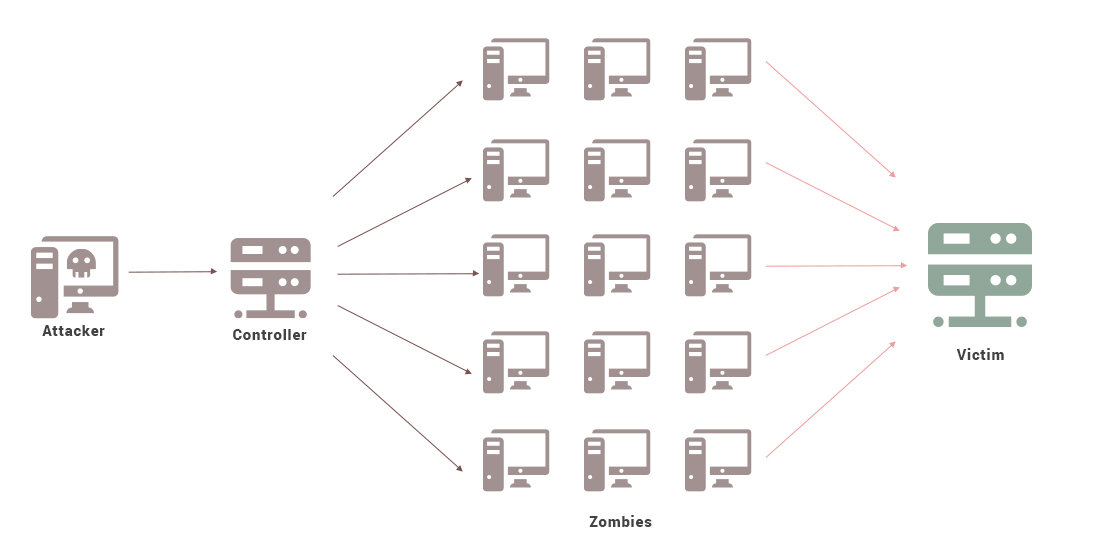
\includegraphics[width=0.75\linewidth]{img/ddos_attack.png}
	\caption{Visualising a DDoS Attack\textsuperscript{\cite{securebox}}}
\end{figure}

In a DDoS attack, the connected devices are usually infected by some sort of malware and operate as part of a botnet. Command and control servers are used to direct the actions of the infected devices in the botnet and dictate what type of attack to launch, data to transmit and what system or network is the target of the attack.

\vspace{0.5cm}

After the first detected DoS attack was launched in the 1970s, DoS and DDoS attacks have remained the most damaging and persistent cyber-attacks to date. One of the first large-scale DDoS attacks occurred in 1999, when a hacker disabled the University of Minnesota's network for over two days. It allowed the attacker to send a DoS instruction to a few command and control servers, which the instructed hundreds of bots to flood the target IP address.

\vspace{0.5cm}

As technology advanced and hackers began to focus more on DDoS attacks, the nature of distributing the attack became significantly more powerful. This ultimately lead to this network attacking technique to become an extremely formidable weapon, and hackers taking on much larger targets.

\begin{figure}[h]
	\centering
	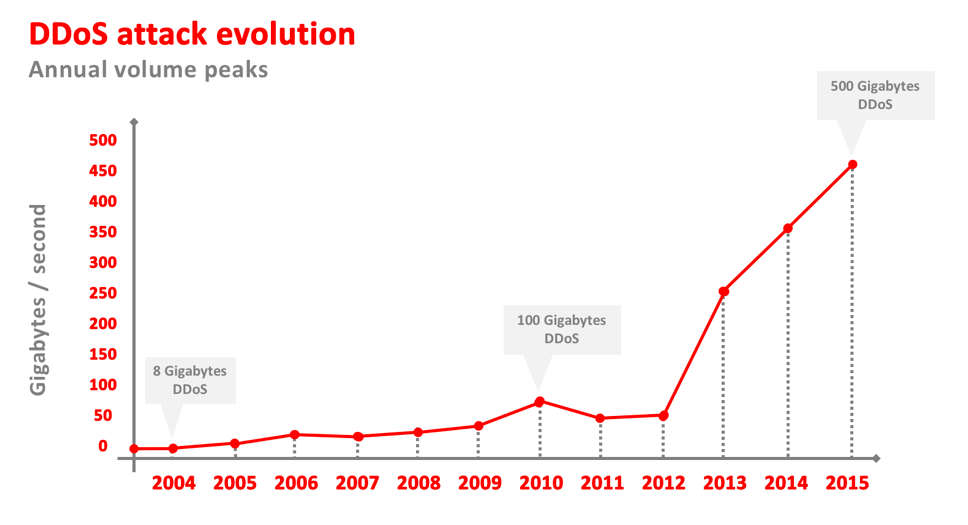
\includegraphics[width=0.75\linewidth]{img/ddos_scale_time.png}
	\caption{DDoS Attack Evolution 2004-15\textsuperscript{\cite{ddosattackevolution}}}
\end{figure}

Recent years have lead to an exponential increase\textsuperscript{\cite{ddosincapsula}} in the number of DDoS attacks, driven by ever-changing motivations and complex, creative ideas.

\vspace{0.5cm}

In 2010 DDoS attacks had become political, with groups such as Anonymous attacking global payment sites. The tool most commonly used in these attacks was known as the Low Orbit Ion Cannon (LOIC). It was originally developed for server stress-testing, but hackers adjusted the software to bring down large servers.

In 2016, DDoS threats evolved to become more materialized. Cyber attacks launched from multiple connected devices were turned into botnets. This propelled the power of attacks to reach around 1TBps of flooding traffic.